% Options for packages loaded elsewhere
\PassOptionsToPackage{unicode}{hyperref}
\PassOptionsToPackage{hyphens}{url}
\PassOptionsToPackage{space}{xeCJK}
%
\documentclass[
  10pt,
  ignorenonframetext,
  aspectratio=169,
  t]{beamer}
\usepackage{pgfpages}
\setbeamertemplate{caption}[numbered]
\setbeamertemplate{caption label separator}{: }
\setbeamercolor{caption name}{fg=normal text.fg}
\beamertemplatenavigationsymbolsempty
% Prevent slide breaks in the middle of a paragraph
\widowpenalties 1 10000
\raggedbottom
\setbeamertemplate{part page}{
  \centering
  \begin{beamercolorbox}[sep=16pt,center]{part title}
    \usebeamerfont{part title}\insertpart\par
  \end{beamercolorbox}
}
\setbeamertemplate{section page}{
  \centering
  \begin{beamercolorbox}[sep=12pt,center]{part title}
    \usebeamerfont{section title}\insertsection\par
  \end{beamercolorbox}
}
\setbeamertemplate{subsection page}{
  \centering
  \begin{beamercolorbox}[sep=8pt,center]{part title}
    \usebeamerfont{subsection title}\insertsubsection\par
  \end{beamercolorbox}
}
\AtBeginPart{
  \frame{\partpage}
}
\AtBeginSection{
  \ifbibliography
  \else
    \frame{\sectionpage}
  \fi
}
\AtBeginSubsection{
  \frame{\subsectionpage}
}
\usepackage{amsmath,amssymb}
\usepackage{iftex}
\ifPDFTeX
  \usepackage[T1]{fontenc}
  \usepackage[utf8]{inputenc}
  \usepackage{textcomp} % provide euro and other symbols
\else % if luatex or xetex
  \usepackage{unicode-math} % this also loads fontspec
  \defaultfontfeatures{Scale=MatchLowercase}
  \defaultfontfeatures[\rmfamily]{Ligatures=TeX,Scale=1}
\fi
\usepackage{lmodern}
\usetheme[]{Madrid}
\usefonttheme{serif} % use mainfont rather than sansfont for slide text
\ifPDFTeX\else
  % xetex/luatex font selection
  \setmainfont[]{DejaVu Sans}
  \setmonofont[]{DejaVu Sans Mono}
  \ifXeTeX
    \usepackage{xeCJK}
    \setCJKmainfont[]{Noto Serif CJK SC}
          \fi
  \ifLuaTeX
    \usepackage[]{luatexja-fontspec}
    \setmainjfont[]{Noto Serif CJK SC}
  \fi
\fi
% Use upquote if available, for straight quotes in verbatim environments
\IfFileExists{upquote.sty}{\usepackage{upquote}}{}
\IfFileExists{microtype.sty}{% use microtype if available
  \usepackage[]{microtype}
  \UseMicrotypeSet[protrusion]{basicmath} % disable protrusion for tt fonts
}{}
\makeatletter
\@ifundefined{KOMAClassName}{% if non-KOMA class
  \IfFileExists{parskip.sty}{%
    \usepackage{parskip}
  }{% else
    \setlength{\parindent}{0pt}
    \setlength{\parskip}{6pt plus 2pt minus 1pt}}
}{% if KOMA class
  \KOMAoptions{parskip=half}}
\makeatother
\usepackage{xcolor}
\newif\ifbibliography
\usepackage{longtable,booktabs,array}
\usepackage{calc} % for calculating minipage widths
\usepackage{caption}
% Make caption package work with longtable
\makeatletter
\def\fnum@table{\tablename~\thetable}
\makeatother
\usepackage{graphicx}
\makeatletter
\def\maxwidth{\ifdim\Gin@nat@width>\linewidth\linewidth\else\Gin@nat@width\fi}
\def\maxheight{\ifdim\Gin@nat@height>\textheight\textheight\else\Gin@nat@height\fi}
\makeatother
% Scale images if necessary, so that they will not overflow the page
% margins by default, and it is still possible to overwrite the defaults
% using explicit options in \includegraphics[width, height, ...]{}
\setkeys{Gin}{width=\maxwidth,height=\maxheight,keepaspectratio}
% Set default figure placement to htbp
\makeatletter
\def\fps@figure{htbp}
\makeatother
\setlength{\emergencystretch}{3em} % prevent overfull lines
\providecommand{\tightlist}{%
  \setlength{\itemsep}{0pt}\setlength{\parskip}{0pt}}
\setcounter{secnumdepth}{-\maxdimen} % remove section numbering
% Tighten vertical rhythm so dense slides fit on a single frame.
\usepackage{etoolbox}
\setlength{\parskip}{3pt plus 1pt minus 1pt}
\setbeamertemplate{itemize/enumerate body begin}{\small}
\setbeamertemplate{itemize/enumerate subbody begin}{\footnotesize}
\AtBeginEnvironment{itemize}{\setlength{\itemsep}{2pt}\setlength{\topsep}{2pt}}
\AtBeginEnvironment{enumerate}{\setlength{\itemsep}{2pt}\setlength{\topsep}{2pt}}
% Shrink code listings and tables so long lines do not force a page break.
\AtBeginEnvironment{Highlighting}{\footnotesize}
\AtBeginEnvironment{verbatim}{\footnotesize}
\AtBeginEnvironment{longtable}{\scriptsize}
\ifLuaTeX
  \usepackage{selnolig}  % disable illegal ligatures
\fi
\IfFileExists{bookmark.sty}{\usepackage{bookmark}}{\usepackage{hyperref}}
\IfFileExists{xurl.sty}{\usepackage{xurl}}{} % add URL line breaks if available
\urlstyle{same}
\hypersetup{
  pdftitle={Terminal-Bench on AgentCore: one image, one Runtime, one microVM per episode},
  pdfauthor={Kaige Yang --- Senior Applied Scientist, AWS},
  hidelinks,
  pdfcreator={LaTeX via pandoc}}

\title[Terminal-Bench on AgentCore]{Terminal-Bench on AgentCore: one image, one Runtime, one microVM
per episode}
\author[Kaige Yang, AWS]{Kaige Yang --- Senior Applied Scientist, AWS}
\date{September 25, 2026}

\setbeamertemplate{frametitle continuation}[from second]
\begin{document}
\frame{\titlepage}

\begin{frame}[fragile]{Summary}
\protect\hypertarget{summary}{}
\begin{longtable}[]{@{}
  >{\raggedright\arraybackslash}p{(\columnwidth - 2\tabcolsep) * \real{0.1522}}
  >{\raggedright\arraybackslash}p{(\columnwidth - 2\tabcolsep) * \real{0.8478}}@{}}
\caption{The deck in one table}\tabularnewline
\toprule\noalign{}
\endfirsthead
\endhead
\textbf{Goal} & RL-train Qwen3-4B (slime GRPO) on Terminal-Bench, every
episode in its own AgentCore microVM \\
\textbf{Challenge} & Isolation needs a \textbf{fresh microVM per
episode}, so every episode pays a \textbf{cold start}, in bursts, at
every step \\
\textbf{Solution} & \textbf{Look-ahead pre-open:} replay slime's data
order and boot the next 2 batches' sessions (P = 64) before slime asks;
heartbeat keeps them alive \\
\textbf{Result} & Smoke run on AWS: 382 episodes, \textbf{0 infra
errors}, \texttt{open\_wait\_ms} \textbf{p95 = 0} (no boot on the
critical path). Cost: ≈ 95 \% of microVM time idle; reward sparse (4
solves) \\
\textbf{Warm-start probe} & Pre-open cuts wait p50 774 → \textbf{5 ms}
(own Runtime) / 1715 → \textbf{0 ms} (Code Interpreter), makespan −20 \%
/ −15 \%. Heartbeat keeps own-Runtime sessions past the idle timeout
(3/3 vs 0/3) \\
\bottomrule\noalign{}
\end{longtable}

Source: \texttt{code/demos/demo\_cpu\_terminalbench/}.
\end{frame}

\begin{frame}[fragile]{Use case · why this demo · design}
\protect\hypertarget{use-case-why-this-demo-design}{}
\begin{longtable}[]{@{}
  >{\raggedright\arraybackslash}p{(\columnwidth - 2\tabcolsep) * \real{0.1522}}
  >{\raggedright\arraybackslash}p{(\columnwidth - 2\tabcolsep) * \real{0.8478}}@{}}
\caption{What this demo covers}\tabularnewline
\toprule\noalign{}
\endfirsthead
\endhead
\textbf{Use case covered} & Tasks that need \textbf{their own OS image}
(packages, \texttt{/etc}, services): hundreds of custom images, one per
task, routed per episode \\
\textbf{Why this demo} & The default Code Interpreter covers most
literature tasks; this is the case it cannot: custom images \textbf{at
scale}, where the cold start is paid per episode \\
\textbf{Isolation} & One episode = one \textbf{brand-new session} = one
dedicated microVM, stopped (VM terminated, memory sanitized) when the
episode ends. Nothing leaks between episodes or GRPO siblings \\
\textbf{Design considerations} & Strict image routing (unmapped task =
error, no fallback) · look-ahead pre-open hides the boot · always-on
heartbeat keeps pre-opened sessions past the 15-min idle timeout · retry
on a new id; infra failures never scored as wrong answers \\
\bottomrule\noalign{}
\end{longtable}
\end{frame}

\hypertarget{setup}{%
\section{1 · Setup}\label{setup}}

\begin{frame}[fragile]{One image → one Runtime → one microVM per
episode}
\protect\hypertarget{one-image-one-runtime-one-microvm-per-episode}{}
\centerline{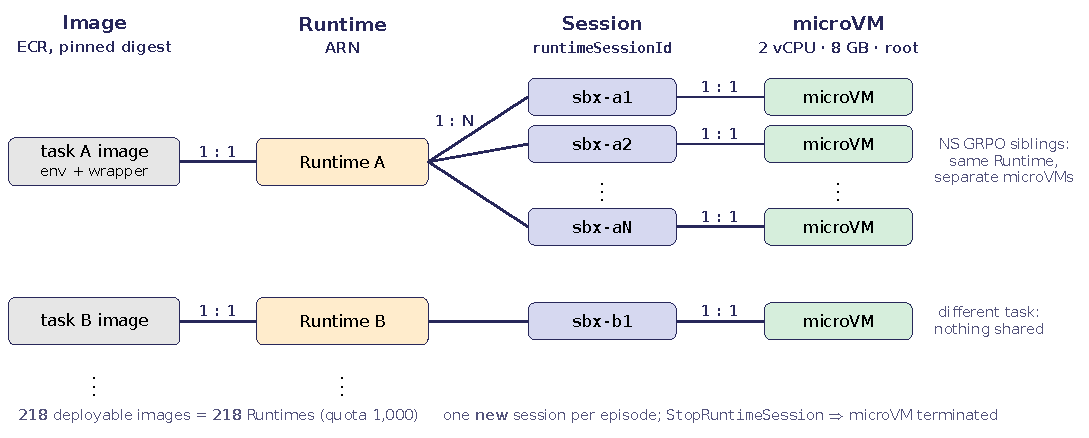
\includegraphics[width=\textwidth,height=0.42\textheight]{figures/tb_fig01_cardinality.pdf}}

\centerline{\emph{Figure 1: image 1:1 Runtime 1:N session 1:1 microVM.}}

\begin{itemize}
\tightlist
\item
  \textbf{Each Terminal-Bench task is its own environment} (OS,
  packages, a deliberately broken state), so each task gets its own
  arm64 image and its own AgentCore Runtime: \textbf{218 Runtimes},
  routed by task id.
\item
  \textbf{Session = microVM, 1:1.} A new \texttt{runtimeSessionId} boots
  a fresh Firecracker VM (2 vCPU, 8 GB) from the pristine image;
  \texttt{StopRuntimeSession} terminates and sanitizes it.
\item
  The image is untouched except for one wrapper layer: a standalone
  Python + a stdlib HTTP server (\texttt{exec}, files, boot timestamps).
  Hidden tests are injected \textbf{after} the agent finishes.
\end{itemize}
\end{frame}

\begin{frame}{The dataset}
\protect\hypertarget{the-dataset}{}
\begin{longtable}[]{@{}
  >{\raggedright\arraybackslash}p{(\columnwidth - 4\tabcolsep) * \real{0.3178}}
  >{\raggedright\arraybackslash}p{(\columnwidth - 4\tabcolsep) * \real{0.1028}}
  >{\raggedright\arraybackslash}p{(\columnwidth - 4\tabcolsep) * \real{0.5794}}@{}}
\caption{From benchmark to training set}\tabularnewline
\toprule\noalign{}
\begin{minipage}[b]{\linewidth}\raggedright
Stage
\end{minipage} & \begin{minipage}[b]{\linewidth}\raggedright
Tasks
\end{minipage} & \begin{minipage}[b]{\linewidth}\raggedright
Dropped because
\end{minipage} \\
\midrule\noalign{}
\endfirsthead
\toprule\noalign{}
\begin{minipage}[b]{\linewidth}\raggedright
Stage
\end{minipage} & \begin{minipage}[b]{\linewidth}\raggedright
Tasks
\end{minipage} & \begin{minipage}[b]{\linewidth}\raggedright
Dropped because
\end{minipage} \\
\midrule\noalign{}
\endhead
Terminal-Bench tasks & 229 & --- \\
Deployable (arm64, ≤ 2 GB image) & \textbf{218} & 7 don't build for
arm64 · 4 exceed the fixed 2 GB image cap \\
Oracle-usable & \textbf{166} & 47 reference solution fails on this
substrate · 5 timed out · 0 pass untouched \\
Train / held-out eval & \textbf{135 / 31} & 80/20, disjoint by task,
stratified by difficulty \\
\bottomrule\noalign{}
\end{longtable}

\begin{itemize}
\tightlist
\item
  \textbf{Oracle check:} keep a task only if the reference solution
  passes \textbf{and} the untouched environment fails; otherwise its
  reward is structurally 0 or 1.
\item
  Images: p50 128 MB, p90 492 MB, max 2 GB (48 GB total). The heavy tail
  (ML models, TeX, toolchains) is what makes boot time vary.
\item
  \textbf{Reward = 1 only if every hidden test passes.}
\end{itemize}
\end{frame}

\begin{frame}[fragile]{How one episode runs}
\protect\hypertarget{how-one-episode-runs}{}
\centerline{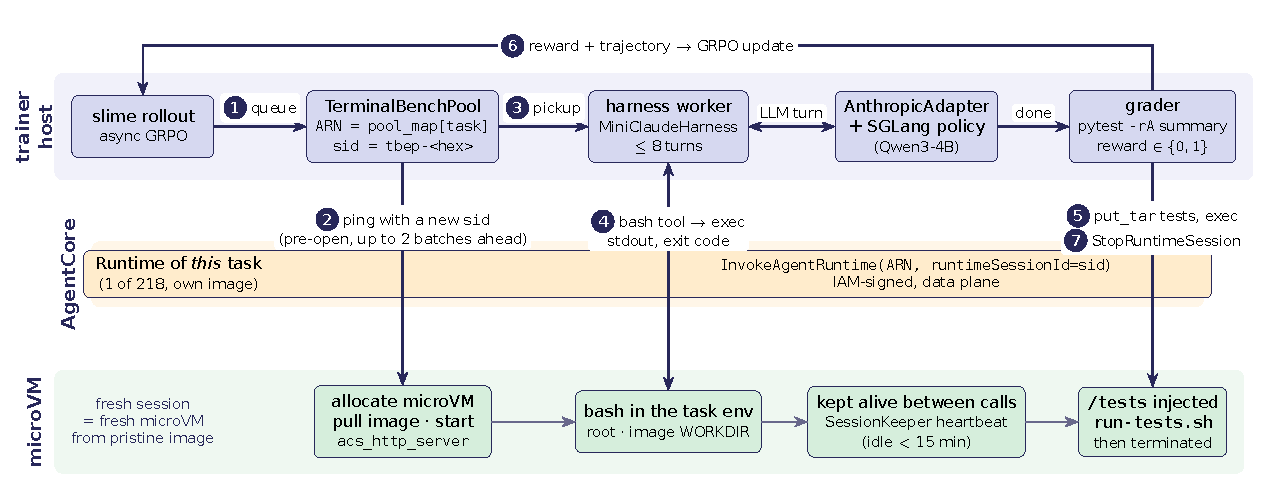
\includegraphics[width=\textwidth,height=0.56\textheight]{figures/tb_fig03_episode-workflow.pdf}}

\centerline{\emph{Figure 2: route → fresh session → agent loop → grade → stop.}}

\begin{itemize}
\tightlist
\item
  There is no ``create session'' call: the first invoke with a new
  \texttt{runtimeSessionId} \textbf{is} the boot.
\item
  One step = RB 4 prompts × NS 8 samples = \textbf{32 episodes = 32
  fresh microVMs}; 4 harness workers run them.
\end{itemize}
\end{frame}

\hypertarget{the-challenge-cold-start}{%
\section{2 · The challenge: cold start}\label{the-challenge-cold-start}}

\begin{frame}[fragile]{Why every episode pays a boot}
\protect\hypertarget{why-every-episode-pays-a-boot}{}
\textbf{We can't reuse a warm VM.} Terminal-Bench tasks change the whole
OS (apt, \texttt{/etc}, services, \texttt{/tmp}). Resetting a workdir
would leak state into the next episode and corrupt the reward and the
GRPO advantage. \textbf{The session is the isolation boundary}, so each
episode needs a new one.

\begin{longtable}[]{@{}
  >{\raggedright\arraybackslash}p{(\columnwidth - 2\tabcolsep) * \real{0.5567}}
  >{\raggedright\arraybackslash}p{(\columnwidth - 2\tabcolsep) * \real{0.4433}}@{}}
\caption{Cold-start cost}\tabularnewline
\toprule\noalign{}
\begin{minipage}[b]{\linewidth}\raggedright
Cost of a fresh session
\end{minipage} & \begin{minipage}[b]{\linewidth}\raggedright
Typical
\end{minipage} \\
\midrule\noalign{}
\endfirsthead
\toprule\noalign{}
\begin{minipage}[b]{\linewidth}\raggedright
Cost of a fresh session
\end{minipage} & \begin{minipage}[b]{\linewidth}\raggedright
Typical
\end{minipage} \\
\midrule\noalign{}
\endhead
Cold boot: allocate VM, pull image, start server & \textbf{≈ 15 s} for a
447 MB image; grows with image size \\
Warm hit: AgentCore already had a spare VM up & ≈ 0.5 s \\
Per step, if on the critical path & 32 × 15 s ≈ \textbf{8 min} of serial
boot \\
\bottomrule\noalign{}
\end{longtable}

\begin{itemize}
\tightlist
\item
  \textbf{Bursty:} all 8 GRPO siblings of a task start at once, on the
  same Runtime.
\item
  \textbf{Idle reclaim:} a session silent for ≈ 15 min is reclaimed, and
  the weight-sync pause can be that long.
\end{itemize}
\end{frame}

\begin{frame}[fragile]{Why the trainer can't hide it on its own}
\protect\hypertarget{why-the-trainer-cant-hide-it-on-its-own}{}
\begin{itemize}
\tightlist
\item
  \textbf{slime only reveals a few episodes at a time:} at most
  \texttt{CONC\ ×\ engines} = 8 \texttt{generate()} calls in flight.
\item
  \textbf{It draws step N+1 only after step N finishes}, so every step's
  first episodes would wait for a boot.
\item
  \textbf{slime knows nothing about sandboxes.} Tasks, Runtimes and
  sessions all live in our \texttt{TerminalBenchPool}, inside slime's
  rollout process.
\end{itemize}

\begin{longtable}[]{@{}
  >{\raggedright\arraybackslash}p{(\columnwidth - 6\tabcolsep) * \real{0.3929}}
  >{\raggedright\arraybackslash}p{(\columnwidth - 6\tabcolsep) * \real{0.1161}}
  >{\raggedright\arraybackslash}p{(\columnwidth - 6\tabcolsep) * \real{0.1518}}
  >{\raggedright\arraybackslash}p{(\columnwidth - 6\tabcolsep) * \real{0.3393}}@{}}
\caption{Options}\tabularnewline
\toprule\noalign{}
\begin{minipage}[b]{\linewidth}\raggedright
Option
\end{minipage} & \begin{minipage}[b]{\linewidth}\raggedright
Hides boot?
\end{minipage} & \begin{minipage}[b]{\linewidth}\raggedright
Keeps isolation?
\end{minipage} & \begin{minipage}[b]{\linewidth}\raggedright
Catch
\end{minipage} \\
\midrule\noalign{}
\endfirsthead
\toprule\noalign{}
\begin{minipage}[b]{\linewidth}\raggedright
Option
\end{minipage} & \begin{minipage}[b]{\linewidth}\raggedright
Hides boot?
\end{minipage} & \begin{minipage}[b]{\linewidth}\raggedright
Keeps isolation?
\end{minipage} & \begin{minipage}[b]{\linewidth}\raggedright
Catch
\end{minipage} \\
\midrule\noalign{}
\endhead
Reuse one warm session per task + reset & ✓ & ✗ & OS state leaks →
\textbf{rejected} \\
Standing warm pool per task & ✓ & ✓ & 218 tasks × NS idle VMs \\
Open on pickup & ✗ & ✓ & Boot on the critical path \\
Fully-async rollout & ✓ & ✓ & Off-policy (stale weights); slime mode
change \\
\textbf{Look-ahead pre-open (used)} & ✓ & ✓ & Guesses can be wrong;
booted VMs idle \\
\bottomrule\noalign{}
\end{longtable}
\end{frame}

\hypertarget{the-solution-look-ahead-pre-open}{%
\section{3 · The solution: look-ahead
pre-open}\label{the-solution-look-ahead-pre-open}}

\begin{frame}[fragile]{Four mechanisms}
\protect\hypertarget{four-mechanisms}{}
\begin{enumerate}
\tightlist
\item
  \textbf{Look-ahead data source.} \texttt{tb\_lookahead\_source.py} (a
  \texttt{-\/-data-source-path} plugin) replays slime's deterministic
  order (sequential offset, \texttt{random.seed(seed\ +\ epoch)}
  shuffle) to list the \textbf{next 2 rollouts'} prompts, without moving
  slime's position. No slime change.
\item
  \textbf{Bounded pre-open window.} The pool keeps a fresh session
  booted for each of the next \textbf{P} = \texttt{TB\_PREOPEN\_BATCHES}
  × RB × NS = \textbf{64} upcoming episodes, pooled per task. A worker
  claims any ready session for its task; the claim moves the window on
  by one. Wrong guesses are stopped at the next draw.
\item
  \textbf{Heartbeat.} A \texttt{SessionKeeper} pings every open session
  at half the 15-min idle timeout, so none is reclaimed during training
  or weight sync.
\item
  \textbf{Retry on a new id.} A failed open retries on a \textbf{new}
  session (3×); an infra failure is logged as \texttt{infra\_error},
  never scored as a wrong answer.
\end{enumerate}

Live microVMs ≤ W + P = 4 + 64 = \textbf{68}. The account quota is
\textbf{5000} active sessions and 25 new/s {[}Q2{]}; throttled opens
back off and retry.
\end{frame}

\begin{frame}{Across a step boundary}
\protect\hypertarget{across-a-step-boundary}{}
\begin{longtable}[]{@{}
  >{\raggedright\arraybackslash}p{(\columnwidth - 4\tabcolsep) * \real{0.3600}}
  >{\raggedright\arraybackslash}p{(\columnwidth - 4\tabcolsep) * \real{0.5280}}
  >{\raggedright\arraybackslash}p{(\columnwidth - 4\tabcolsep) * \real{0.1120}}@{}}
\caption{Look-ahead across a step boundary (W = 4, P =
64)}\tabularnewline
\toprule\noalign{}
\begin{minipage}[b]{\linewidth}\raggedright
Moment
\end{minipage} & \begin{minipage}[b]{\linewidth}\raggedright
What happens
\end{minipage} & \begin{minipage}[b]{\linewidth}\raggedright
Worker waits for a boot?
\end{minipage} \\
\midrule\noalign{}
\endfirsthead
\toprule\noalign{}
\begin{minipage}[b]{\linewidth}\raggedright
Moment
\end{minipage} & \begin{minipage}[b]{\linewidth}\raggedright
What happens
\end{minipage} & \begin{minipage}[b]{\linewidth}\raggedright
Worker waits for a boot?
\end{minipage} \\
\midrule\noalign{}
\endhead
Step N−1 running & Its draw already announced steps N and N+1 → 64
sessions booting & --- \\
Step N drawn & Window = steps N, N+1: already booted, nothing new to
open & --- \\
Each claim & Next episode of step N+2 starts booting & \textbf{No} \\
Step N training & 64 booted VMs idle through training; heartbeat keeps
them & --- \\
Step N+1 drawn & All its episodes already booted & \textbf{No} \\
\bottomrule\noalign{}
\end{longtable}

\begin{itemize}
\tightlist
\item
  \textbf{Sessions per Runtime are never configured.} A task sampled in
  a step gets NS = 8 sessions; others get 0.
\item
  \textbf{The price is idle time:} each VM is booted about P · E / W
  seconds before it's needed (E = episode time).
\end{itemize}
\end{frame}

\begin{frame}[fragile]{Sizing \texttt{TB\_PREOPEN\_BATCHES}}
\protect\hypertarget{sizing-tb_preopen_batches}{}
Boot is hidden when \textbf{P · E / W ≥ B} (B = boot time), and a window
of at least one batch (P ≥ RB × NS) also covers each step's first
episodes. Everything beyond that is paid idle time.

\begin{longtable}[]{@{}
  >{\raggedright\arraybackslash}p{(\columnwidth - 6\tabcolsep) * \real{0.2653}}
  >{\raggedright\arraybackslash}p{(\columnwidth - 6\tabcolsep) * \real{0.0612}}
  >{\raggedright\arraybackslash}p{(\columnwidth - 6\tabcolsep) * \real{0.3673}}
  >{\raggedright\arraybackslash}p{(\columnwidth - 6\tabcolsep) * \real{0.3061}}@{}}
\caption{Choosing TB\_PREOPEN\_BATCHES}\tabularnewline
\toprule\noalign{}
\begin{minipage}[b]{\linewidth}\raggedright
\texttt{TB\_PREOPEN\_BATCHES}
\end{minipage} & \begin{minipage}[b]{\linewidth}\raggedright
P
\end{minipage} & \begin{minipage}[b]{\linewidth}\raggedright
Boot hidden?
\end{minipage} & \begin{minipage}[b]{\linewidth}\raggedright
Idle per VM ≈ P · E / W
\end{minipage} \\
\midrule\noalign{}
\endfirsthead
\toprule\noalign{}
\begin{minipage}[b]{\linewidth}\raggedright
\texttt{TB\_PREOPEN\_BATCHES}
\end{minipage} & \begin{minipage}[b]{\linewidth}\raggedright
P
\end{minipage} & \begin{minipage}[b]{\linewidth}\raggedright
Boot hidden?
\end{minipage} & \begin{minipage}[b]{\linewidth}\raggedright
Idle per VM ≈ P · E / W
\end{minipage} \\
\midrule\noalign{}
\endhead
0 --- look-ahead off & ≈ 4 & Mid-step only; each step's first W wait & ≈
20 s \\
1 --- one batch ahead & 32 & Yes, including step starts & ≈ 3 min \\
\textbf{2 --- used in the smoke run} & \textbf{64} & Yes, with a full
batch of slack & ≈ 6 min (measured: 7.3 min p50) \\
\bottomrule\noalign{}
\end{longtable}

E = 21 s (measured episode p50), W = 4. Tune from the
\texttt{{[}demo{]}} lines: \texttt{open\_wait\_ms} ≫ 0 → raise it;
\texttt{preopen\_idle\_ms} ≫ boot time → lower it.
\end{frame}

\hypertarget{results}{%
\section{4 · Results}\label{results}}

\begin{frame}[fragile]{Smoke run: learning (10 steps + eval,
2026-09-23)}
\protect\hypertarget{smoke-run-learning-10-steps-eval-2026-09-23}{}
\begin{longtable}[]{@{}
  >{\raggedright\arraybackslash}p{(\columnwidth - 2\tabcolsep) * \real{0.3137}}
  >{\raggedright\arraybackslash}p{(\columnwidth - 2\tabcolsep) * \real{0.6863}}@{}}
\caption{Learning (RB = 4, NS = 8, Qwen3-4B)}\tabularnewline
\toprule\noalign{}
\begin{minipage}[b]{\linewidth}\raggedright
Metric
\end{minipage} & \begin{minipage}[b]{\linewidth}\raggedright
Value
\end{minipage} \\
\midrule\noalign{}
\endfirsthead
\toprule\noalign{}
\begin{minipage}[b]{\linewidth}\raggedright
Metric
\end{minipage} & \begin{minipage}[b]{\linewidth}\raggedright
Value
\end{minipage} \\
\midrule\noalign{}
\endhead
Train solve rate, steps 1--10 & 0 · 0 · 0.088 · 0 · 0 · 0 · 0 · 0.026 ·
0 · 0 \\
Full solves & \textbf{4 / 382} episodes
(\texttt{acl-permissions-inheritance} ×3, \texttt{git-leak-recovery}) \\
Held-out solve rate (31 tasks × 2) & 0.0 \\
Partial progress & \textbf{42 \%} of episodes pass ≥ 1 hidden test \\
Agent behaviour & Median 6 turns, 5 bash calls; 45 \% hit the 8-turn
budget \\
\bottomrule\noalign{}
\end{longtable}

\begin{itemize}
\tightlist
\item
  \textbf{Sparse, not dead.} The tool loop works and the agent makes
  partial progress, but almost every GRPO group is all-0, so there is
  little gradient.
\end{itemize}
\end{frame}

\begin{frame}[fragile]{Smoke run: sandbox and cost}
\protect\hypertarget{smoke-run-sandbox-and-cost}{}
\begin{longtable}[]{@{}
  >{\raggedright\arraybackslash}p{(\columnwidth - 2\tabcolsep) * \real{0.3711}}
  >{\raggedright\arraybackslash}p{(\columnwidth - 2\tabcolsep) * \real{0.6289}}@{}}
\caption{Sandbox and cost (W = 4, TB\_PREOPEN\_BATCHES =
2)}\tabularnewline
\toprule\noalign{}
\begin{minipage}[b]{\linewidth}\raggedright
Metric
\end{minipage} & \begin{minipage}[b]{\linewidth}\raggedright
Value
\end{minipage} \\
\midrule\noalign{}
\endfirsthead
\toprule\noalign{}
\begin{minipage}[b]{\linewidth}\raggedright
Metric
\end{minipage} & \begin{minipage}[b]{\linewidth}\raggedright
Value
\end{minipage} \\
\midrule\noalign{}
\endhead
Episodes / infra errors & 382, each on its own fresh microVM /
\textbf{0} lost (job ≈ 70 min) \\
Boot on the critical path (\texttt{open\_wait\_ms}) & \textbf{p50 0 ·
p95 0}; max 4.9 s (first 4 episodes only) \\
Session open (\texttt{open\_ms}) & p50 0.66 s · p95 2.5 s · \textbf{100
\% warm hits} · 0 retries \\
Episode time p50 / p90 & 21 s / 64 s (agent 9 s + grade 10 s) \\
Pre-opened VM idle p50 / max & \textbf{7.3 min} / 16.5 min; heartbeat
kept all alive \\
microVM-seconds per train step & ≈ 13 000 (32 × 411 s); \textbf{≈ 95 \%
idle} \\
\bottomrule\noalign{}
\end{longtable}

\begin{itemize}
\tightlist
\item
  \textbf{Every open was a warm hit.} AgentCore already had a spare VM
  up for each Runtime, so no ≈ 15 s cold boot occurred in this run. The
  per-image cold-start probe (\texttt{probe\_coldstart.py}) is still to
  run.
\end{itemize}
\end{frame}

\begin{frame}[fragile]{Warm-start probe: pre-open (\texttt{warmstart/},
2026-09-25)}
\protect\hypertarget{warm-start-probe-pre-open-warmstart-2026-09-25}{}
Host-only, no GPU or trainer (≈ 7 min, a few cents): the same 24
MockPolicy \texttt{sql} episodes in batches of 6, \textbf{cold} (open at
episode start) vs \textbf{preopen} (next batch booted while this one
runs, the \texttt{TB\_PREOPEN\_BATCHES} idea).

\begin{longtable}[]{@{}
  >{\raggedright\arraybackslash}p{(\columnwidth - 10\tabcolsep) * \real{0.2222}}
  >{\raggedright\arraybackslash}p{(\columnwidth - 10\tabcolsep) * \real{0.1111}}
  >{\raggedleft\arraybackslash}p{(\columnwidth - 10\tabcolsep) * \real{0.1222}}
  >{\raggedleft\arraybackslash}p{(\columnwidth - 10\tabcolsep) * \real{0.2333}}
  >{\raggedleft\arraybackslash}p{(\columnwidth - 10\tabcolsep) * \real{0.1111}}
  >{\raggedleft\arraybackslash}p{(\columnwidth - 10\tabcolsep) * \real{0.2000}}@{}}
\caption{Pre-open vs cold open (all rewards 1.0)}\tabularnewline
\toprule\noalign{}
\begin{minipage}[b]{\linewidth}\raggedright
Backend
\end{minipage} & \begin{minipage}[b]{\linewidth}\raggedright
Mode
\end{minipage} & \begin{minipage}[b]{\linewidth}\raggedleft
Wait p50
\end{minipage} & \begin{minipage}[b]{\linewidth}\raggedleft
Episodes that waited
\end{minipage} & \begin{minipage}[b]{\linewidth}\raggedleft
Idle held
\end{minipage} & \begin{minipage}[b]{\linewidth}\raggedleft
Makespan
\end{minipage} \\
\midrule\noalign{}
\endfirsthead
\toprule\noalign{}
\begin{minipage}[b]{\linewidth}\raggedright
Backend
\end{minipage} & \begin{minipage}[b]{\linewidth}\raggedright
Mode
\end{minipage} & \begin{minipage}[b]{\linewidth}\raggedleft
Wait p50
\end{minipage} & \begin{minipage}[b]{\linewidth}\raggedleft
Episodes that waited
\end{minipage} & \begin{minipage}[b]{\linewidth}\raggedleft
Idle held
\end{minipage} & \begin{minipage}[b]{\linewidth}\raggedleft
Makespan
\end{minipage} \\
\midrule\noalign{}
\endhead
Own Runtime & cold & 774 ms & 24 / 24 & 0 s & 31.9 s \\
Own Runtime & preopen & \textbf{5 ms} & 8 / 24 (first batch) & 75 s &
25.5 s (\textbf{−20 \%}) \\
Code Interpreter & cold & 1715 ms & 24 / 24 & 0 s & 28.7 s \\
Code Interpreter & preopen & \textbf{0 ms} & 6 / 24 (first batch) & 70 s
& 24.3 s (\textbf{−15 \%}) \\
\bottomrule\noalign{}
\end{longtable}

\begin{itemize}
\tightlist
\item
  \textbf{Only the first batch pays the boot.} The price is ``idle
  held'', the same trade-off \texttt{preopen\_idle\_ms} shows at full
  scale.
\end{itemize}
\end{frame}

\begin{frame}[fragile]{Warm-start probe: heartbeat}
\protect\hypertarget{warm-start-probe-heartbeat}{}
A Runtime session idle past \texttt{idleRuntimeSessionTimeout} is
reclaimed. In training that timeout is the \textbf{15-min default}
(\texttt{WARM\_IDLE\_TIMEOUT} = 900, pings at 450 s). The probe Runtime
\texttt{acs\_warmstart\_cpu} sets it to \textbf{60 s} only so the test
fits in minutes; sessions then sit idle 150 s.

\begin{longtable}[]{@{}
  >{\raggedright\arraybackslash}p{(\columnwidth - 6\tabcolsep) * \real{0.2222}}
  >{\raggedright\arraybackslash}p{(\columnwidth - 6\tabcolsep) * \real{0.1889}}
  >{\raggedleft\arraybackslash}p{(\columnwidth - 6\tabcolsep) * \real{0.1111}}
  >{\raggedright\arraybackslash}p{(\columnwidth - 6\tabcolsep) * \real{0.4778}}@{}}
\caption{Heartbeat vs idle reclaim}\tabularnewline
\toprule\noalign{}
\begin{minipage}[b]{\linewidth}\raggedright
Backend
\end{minipage} & \begin{minipage}[b]{\linewidth}\raggedright
Heartbeat
\end{minipage} & \begin{minipage}[b]{\linewidth}\raggedleft
Sessions surviving the idle gap
\end{minipage} & \begin{minipage}[b]{\linewidth}\raggedright
Resume
\end{minipage} \\
\midrule\noalign{}
\endfirsthead
\toprule\noalign{}
\begin{minipage}[b]{\linewidth}\raggedright
Backend
\end{minipage} & \begin{minipage}[b]{\linewidth}\raggedright
Heartbeat
\end{minipage} & \begin{minipage}[b]{\linewidth}\raggedleft
Sessions surviving the idle gap
\end{minipage} & \begin{minipage}[b]{\linewidth}\raggedright
Resume
\end{minipage} \\
\midrule\noalign{}
\endhead
Own Runtime & on (14 pings) & \textbf{3 / 3} & 104 ms, files intact \\
Own Runtime & off & 0 / 3 & \textbf{Silently reclaimed:} same session
id, fresh empty sandbox \\
Code Interpreter & on / off & 0 / 3 & Ends at its
\texttt{sessionTimeoutSeconds} regardless of pings \\
\bottomrule\noalign{}
\end{longtable}

\begin{itemize}
\tightlist
\item
  \textbf{Why the keeper is always on here:} a reclaimed session looks
  healthy but has lost its files. On the Code Interpreter the lever is a
  generous session timeout, not pings.
\end{itemize}
\end{frame}

\begin{frame}[fragile]{Takeaways and next steps}
\protect\hypertarget{takeaways-and-next-steps}{}
\begin{itemize}
\tightlist
\item
  \textbf{Works end to end:} per-task Runtimes, one fresh microVM per
  episode, oracle-checked tasks, 0 infra failures.
\item
  \textbf{Cold start is solved, but over-provisioned.} Look-ahead
  removed all boot wait (the warm-start probe confirms: only the first
  batch waits), but at P = 64 a VM idles ≈ 7 min for a 21 s episode.
  With warm hits at ≈ 0.7 s, \textbf{\texttt{TB\_PREOPEN\_BATCHES} = 1
  (or 0)} should give the same wait at a fraction of the cost.
\item
  \textbf{Learning signal is the bottleneck:} 4 solves in 382 episodes.
  Next: easy-first curriculum, more turns, or partial credit from
  \texttt{tests\_passed}.
\end{itemize}

\begin{longtable}[]{@{}
  >{\raggedright\arraybackslash}p{(\columnwidth - 2\tabcolsep) * \real{0.4433}}
  >{\raggedright\arraybackslash}p{(\columnwidth - 2\tabcolsep) * \real{0.5567}}@{}}
\caption{Next steps}\tabularnewline
\toprule\noalign{}
\begin{minipage}[b]{\linewidth}\raggedright
Next
\end{minipage} & \begin{minipage}[b]{\linewidth}\raggedright
Why
\end{minipage} \\
\midrule\noalign{}
\endfirsthead
\toprule\noalign{}
\begin{minipage}[b]{\linewidth}\raggedright
Next
\end{minipage} & \begin{minipage}[b]{\linewidth}\raggedright
Why
\end{minipage} \\
\midrule\noalign{}
\endhead
Re-run with \texttt{TB\_PREOPEN\_BATCHES} = 1 and 0 & Measure the
cost/wait trade-off \\
\texttt{probe\_coldstart.py} over all 218 Runtimes & Cold vs warm boot
by image size (burst opens) \\
Curriculum / partial-credit reward & Mixed GRPO groups → real
gradient \\
\bottomrule\noalign{}
\end{longtable}
\end{frame}

\begin{frame}[fragile]{References}
\protect\hypertarget{references}{}
\begin{longtable}[]{@{}
  >{\raggedright\arraybackslash}p{(\columnwidth - 4\tabcolsep) * \real{0.0545}}
  >{\raggedright\arraybackslash}p{(\columnwidth - 4\tabcolsep) * \real{0.5455}}
  >{\raggedright\arraybackslash}p{(\columnwidth - 4\tabcolsep) * \real{0.4000}}@{}}
\caption{References}\tabularnewline
\toprule\noalign{}
\begin{minipage}[b]{\linewidth}\raggedright
Ref
\end{minipage} & \begin{minipage}[b]{\linewidth}\raggedright
Source
\end{minipage} & \begin{minipage}[b]{\linewidth}\raggedright
Supports
\end{minipage} \\
\midrule\noalign{}
\endfirsthead
\toprule\noalign{}
\begin{minipage}[b]{\linewidth}\raggedright
Ref
\end{minipage} & \begin{minipage}[b]{\linewidth}\raggedright
Source
\end{minipage} & \begin{minipage}[b]{\linewidth}\raggedright
Supports
\end{minipage} \\
\midrule\noalign{}
\endhead
{[}Q1{]} & AgentCore quotas:
\url{https://docs.aws.amazon.com/bedrock-agentcore/latest/devguide/bedrock-agentcore-limits.html}
& 1000 Runtimes/account · image ≤ 2 GB · 15-min request timeout · 15-min
idle timeout \\
{[}Q2{]} &
\texttt{aws\ service-quotas\ list-service-quotas\ -\/-service-code\ bedrock-agentcore}
(us-west-2, 2026-09-23) & Active Session Workloads = 5000 (L-3E5722B2) ·
new sessions 25/s (L-8EE2AEA2) · image 2048 MB (L-0A9E32B3) \\
{[}D3{]} &
\url{https://docs.aws.amazon.com/bedrock-agentcore/latest/devguide/runtime-how-it-works.html}
& Session = dedicated microVM; 15-min idle, 8 h max lifetime \\
\bottomrule\noalign{}
\end{longtable}
\end{frame}

\end{document}
